\documentclass[tikz,border=5pt]{standalone}
\usepackage[T1]{fontenc}
\usepackage{lmodern,amsmath,amssymb}
\usetikzlibrary{arrows.meta,calc,positioning,fit,backgrounds,shapes.geometric,matrix,decorations.pathreplacing,patterns}
\definecolor{ink}{gray}{0.08}
\definecolor{wash}{gray}{0.965}
\definecolor{soft}{gray}{0.45}
\tikzset{box/.style={draw=ink,line width=.65pt,fill=white,align=center,inner sep=4pt,outer sep=0pt,font=\small},flow/.style={draw=ink,line width=.65pt,-{Latex[length=1.8mm,width=1.3mm]},rounded corners=2pt},annotation/.style={font=\scriptsize,text=soft,align=center},groupbox/.style={draw=soft,dashed,line width=.45pt,fill=wash}}
\begin{document}
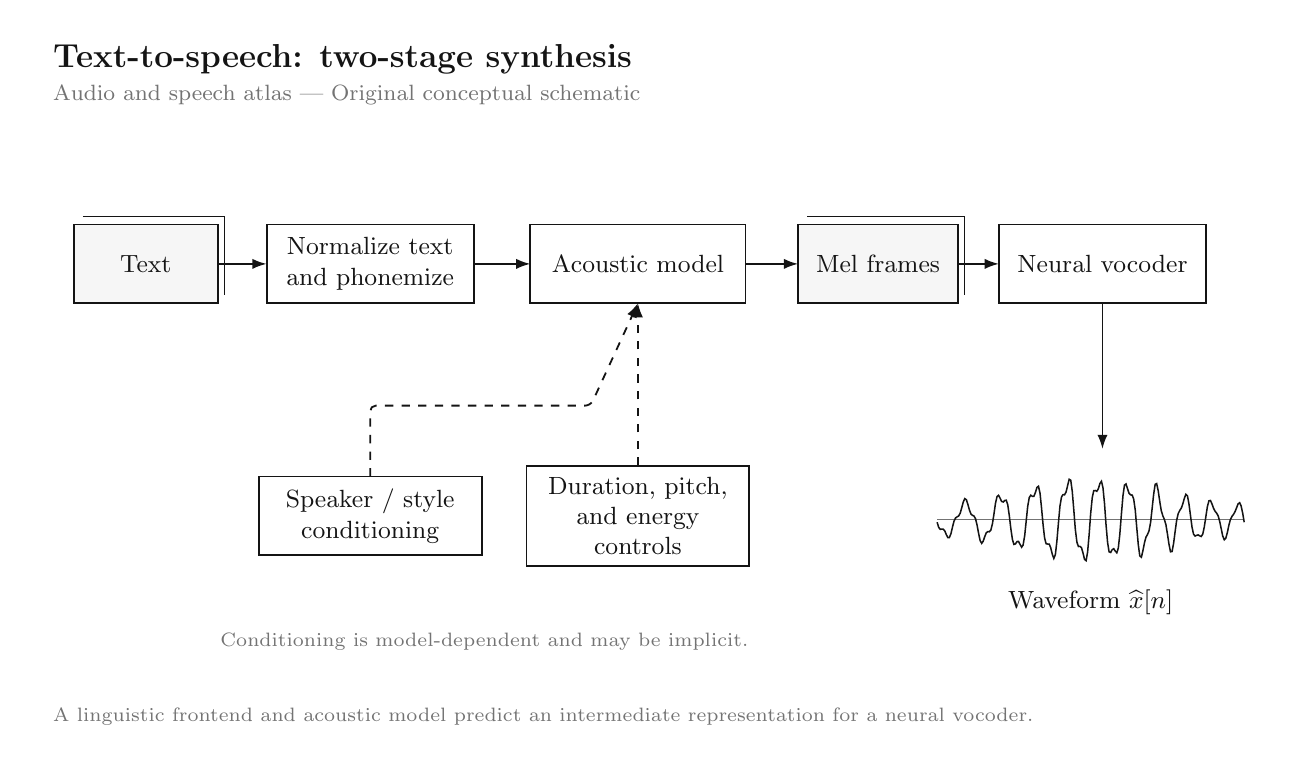
\begin{tikzpicture}[x=1cm,y=-1cm,font=\rmfamily,text=ink]

\path[use as bounding box] (0,0) rectangle (16,9);
\node[anchor=west,font=\large\bfseries] at (.2,.4) {Text-to-speech: two-stage synthesis};
\node[anchor=west,font=\footnotesize,text=soft] at (.2,.85) {Audio and speech atlas | Original conceptual schematic};
\begin{pgfonlayer}{background}
\end{pgfonlayer}
\node[box,fill=wash,minimum width=1.8cm,minimum height=1.0cm,text width=1.55cm] (text) at (1.5,3.0) {Text};
\draw[ink,line width=.4pt] (0.7,2.4) -- (2.5,2.4) -- (2.5,3.4);
\node[box,minimum width=2.6cm,minimum height=1.0cm,text width=2.35cm] (front) at (4.35,3.0) {Normalize text\\and phonemize};
\node[box,minimum width=2.7cm,minimum height=1.0cm,text width=2.45cm] (acoustic) at (7.75,3.0) {Acoustic model};
\node[box,fill=wash,minimum width=2.0cm,minimum height=1.0cm,text width=1.75cm] (mel) at (10.8,3.0) {Mel frames};
\draw[ink,line width=.4pt] (9.9,2.4) -- (11.9,2.4) -- (11.9,3.4);
\node[box,minimum width=2.6cm,minimum height=1.0cm,text width=2.35cm] (vocoder) at (13.65,3.0) {Neural vocoder};
\node[box,minimum width=2.8cm,minimum height=1.0cm,text width=2.55cm] (speaker) at (4.35,6.2) {Speaker / style\\conditioning};
\node[box,minimum width=2.8cm,minimum height=1.0cm,text width=2.55cm] (prosody) at (7.75,6.2) {Duration, pitch,\\and energy controls};
\begin{pgfonlayer}{background}
\draw[flow] (text.east) -- (front.west);
\draw[flow] (front.east) -- (acoustic.west);
\draw[flow] (acoustic.east) -- (mel.west);
\draw[flow] (mel.east) -- (vocoder.west);
\draw[flow,dashed] (speaker.north) -- (4.35,4.8) -- (7.15,4.8) -- (acoustic.south);
\draw[flow,dashed] (prosody.north) -- (acoustic.south);
\end{pgfonlayer}
\draw[soft,line width=.35pt] (11.55,6.25) -- (15.450000000000001,6.25);
\draw[ink,line width=.55pt] plot coordinates {(11.550,6.281) (11.570,6.346) (11.589,6.371) (11.609,6.368) (11.628,6.369) (11.648,6.393) (11.667,6.439) (11.687,6.477) (11.706,6.475) (11.726,6.424) (11.745,6.343) (11.764,6.268) (11.784,6.226) (11.804,6.212) (11.823,6.202) (11.843,6.166) (11.862,6.099) (11.882,6.024) (11.901,5.981) (11.921,5.994) (11.940,6.053) (11.960,6.125) (11.979,6.175) (11.998,6.193) (12.018,6.202) (12.038,6.237) (12.057,6.317) (12.077,6.424) (12.096,6.514) (12.116,6.549) (12.135,6.522) (12.155,6.463) (12.174,6.415) (12.194,6.400) (12.213,6.402) (12.232,6.381) (12.252,6.303) (12.272,6.175) (12.291,6.041) (12.311,5.954) (12.330,5.939) (12.350,5.976) (12.369,6.017) (12.389,6.024) (12.408,6.005) (12.428,6.001) (12.447,6.060) (12.466,6.193) (12.486,6.361) (12.506,6.499) (12.525,6.563) (12.545,6.556) (12.564,6.526) (12.584,6.525) (12.603,6.562) (12.623,6.598) (12.642,6.571) (12.662,6.452) (12.681,6.266) (12.700,6.082) (12.720,5.967) (12.740,5.938) (12.759,5.952) (12.779,5.951) (12.798,5.903) (12.818,5.838) (12.837,5.824) (12.857,5.914) (12.876,6.100) (12.896,6.317) (12.915,6.482) (12.934,6.554) (12.954,6.558) (12.974,6.559) (12.993,6.607) (13.013,6.690) (13.032,6.741) (13.052,6.690) (13.071,6.520) (13.091,6.285) (13.110,6.075) (13.130,5.959) (13.149,5.931) (13.168,5.932) (13.188,5.896) (13.208,5.812) (13.227,5.735) (13.247,5.747) (13.266,5.889) (13.286,6.128) (13.305,6.371) (13.325,6.533) (13.344,6.589) (13.364,6.588) (13.383,6.603) (13.402,6.670) (13.422,6.752) (13.442,6.769) (13.461,6.659) (13.481,6.432) (13.500,6.169) (13.520,5.968) (13.539,5.880) (13.559,5.878) (13.578,5.888) (13.598,5.855) (13.617,5.790) (13.637,5.761) (13.656,5.841) (13.676,6.046) (13.695,6.312) (13.715,6.540) (13.734,6.657) (13.754,6.665) (13.773,6.629) (13.793,6.617) (13.812,6.647) (13.832,6.669) (13.851,6.609) (13.870,6.434) (13.890,6.182) (13.910,5.946) (13.929,5.810) (13.949,5.795) (13.968,5.855) (13.988,5.915) (14.007,5.934) (14.027,5.936) (14.046,5.985) (14.066,6.126) (14.085,6.346) (14.105,6.569) (14.124,6.709) (14.144,6.725) (14.163,6.645) (14.183,6.542) (14.202,6.471) (14.222,6.436) (14.241,6.390) (14.261,6.284) (14.280,6.111) (14.300,5.924) (14.319,5.800) (14.338,5.790) (14.358,5.884) (14.378,6.021) (14.397,6.135) (14.417,6.201) (14.436,6.245) (14.456,6.314) (14.475,6.430) (14.495,6.564) (14.514,6.656) (14.534,6.652) (14.553,6.550) (14.573,6.396) (14.592,6.256) (14.612,6.170) (14.631,6.132) (14.651,6.102) (14.670,6.048) (14.690,5.976) (14.709,5.926) (14.729,5.945) (14.748,6.047) (14.768,6.199) (14.787,6.342) (14.806,6.431) (14.826,6.456) (14.846,6.447) (14.865,6.442) (14.885,6.454) (14.904,6.462) (14.924,6.430) (14.943,6.340) (14.963,6.209) (14.982,6.083) (15.002,6.009) (15.021,6.005) (15.041,6.049) (15.060,6.103) (15.080,6.141) (15.099,6.165) (15.119,6.200) (15.138,6.268) (15.158,6.364) (15.177,6.456) (15.197,6.504) (15.216,6.484) (15.236,6.411) (15.255,6.320) (15.274,6.248) (15.294,6.207) (15.314,6.181) (15.333,6.147) (15.353,6.097) (15.372,6.048) (15.392,6.033) (15.411,6.075) (15.431,6.169) (15.450,6.281)};
\draw[flow] (13.65,3.5) -- (13.65,5.35);
\node[align=center,anchor=center,font=\small,text=ink,text width=3.7cm] at (13.5,7.3) {Waveform \mbox{$\widehat{x}[n]$}};
\node[align=center,anchor=center,font=\scriptsize,text=soft,text width=8cm] at (5.8,7.8) {Conditioning is model-dependent and may be implicit.};
\node[anchor=west,align=left,font=\scriptsize,text=soft,text width=15.6cm] at (.2,8.75) {A linguistic frontend and acoustic model predict an intermediate representation for a neural vocoder.};
\end{tikzpicture}
\end{document}
